\documentclass[11pt,          % font size: 11pt or 12pt
               phd,            % degree:    ms or phd
               %hardcopy,     % prepare document for hardcopy printing
                              %  Don't enable for ETD submission.
               onehalfspacing % spacing: onehalfspacing or doublespacing
               ]{ncsuthesis}

%%----------------------------------------------------------------------------%%
%%------------------------------ Import Packages -----------------------------%%
%%----------------------------------------------------------------------------%%

\usepackage{booktabs}  % professionally typeset tables
\usepackage{amsmath}
\usepackage{xcolor}
\usepackage{lipsum}    % filler text


%%----------------------------------------------------------------------------%%
%%-------------------------------- Fonts -------------------------------------%%
%%----------------------------------------------------------------------------%%

%% ETD guidelines don't specify the font.  You can enable the fonts
%% by uncommenting the appropriate lines.
%% See http://www.tug.dk/FontCatalogue/ for more options.

%% Serif Fonts -------------------------------------------------
%%  The four serif fonts listed here (Utopia, Palatino, Kerkis,
%%  and Times) all have math support.
%%  Uncomment one of the below if you would like to switch to
%%  something other than the default Computer Modern.

%% Utopia
%\usepackage[T1]{fontenc}
%\usepackage[adobe-utopia]{mathdesign}

%% Palatino
%\usepackage[T1]{fontenc}
%\usepackage[sc]{mathpazo}
%\linespread{1.05}

%% Kerkis
%\usepackage[T1]{fontenc}
%\usepackage{kmath,kerkis}

%% Times
%\usepackage[T1]{fontenc}
%\usepackage{mathptmx}

%% Sans serif fonts -------------------------

%\usepackage[scaled]{helvet}  % Helvetica
%\usepackage[scaled]{berasans} % Bera Sans




%%----------------------------------------------------------------------------%%
%%---------------------------- Formatting Options ----------------------------%%
%%----------------------------------------------------------------------------%%
%%

%% -------------------------------------------------------------------------- %%
%% Disposition format -- any titles, headings, section titles
%%  These formatting commands affect all headings, titles, headings,
%%  so sizing commands should not be used here.
%%  Formatting options to consider are
%%     +  \sffamily - sans serif fonts.  Dispositions are often typeset in
%%                    sans serif, so this is a good option. 
%%     +  \rmfamily - serif fonts
%%     +  \bfseries - bold face
%\dispositionformat{\sffamily\bfseries}   % bold and sans serif
\dispositionformat{\bfseries}            % bold and serif

%% Formatting for centered headings - Abstract, Dedication, etc. headings
%%  This is where one might put a sizing command.
%%  \MakeUppercase can be used to typeset all headings in uppercase.
\headingformat{\large\MakeUppercase}   % All letters uppercase
%\headingformat{\large}                % Not all uppercase
%\headingformat{\Large\scshape}        % Small Caps, used with serif fonts.


%%----------------------------------------------------------------------------%%
%%---------------------------- Content Options -------------------------------%%
%%----------------------------------------------------------------------------%%
%% Size of committee: 3 or 4
%\committeesize{3}
\committeesize{4}

%% Members of committee
\chair{Doug Dodd}
\memberI{Alex Anderson}
\memberII{Bobby Brown}
\memberIII{Chris Cox} % unnecessary if committeesize=3

%% Student writing thesis, first middle last
\student{John}{Mark}{Smith}

%% Degree program
\program{Nuclear Engineering}

%% Thesis Title
%%  Keep in mind, according to ETD guidelines:
%%    +  Capitalize first letter of important words.
%%    +  Use inverted pyramid shape if title spans more than one line.
%%
%%  Note: To break the title onto multiple lines, use \break instead of \\.
\thesistitle{A North Carolina State University Sample \LaTeX{} Thesis \break 
with a Title So Long it Needs a Line Break}

%% Hyperref package creates PDF metadata and hyperlinks in Table of Contents
%%  and citations.  You don't have to use this package if you don't want it.
\usepackage[
  pdfauthor={John Mark Smith},
  pdftitle={The Title},
  pdfcreator={pdftex},
  pdfsubject={NC State ETD Thesis},
  pdfkeywords={keyword1, keyword2},
  colorlinks=true,
  linkcolor=black,
  citecolor=black,
]{hyperref}

%%----------------------------------------------------------------------------%%
%%---------------------------- Personal Macros -------------------------------%%
%%----------------------------------------------------------------------------%%

%% A central location to add your favorite macros.

%% A few examples to get you started.
\newcommand{\uv}[1]{\ensuremath{\mathbf{\hat{#1}}}}
\newcommand{\bo}{\ensuremath{\boldsymbol{\Omega}}}
\newcommand{\eref}[1]{Eq.~\ref{#1}}
\newcommand{\fref}[1]{Figure~\ref{#1}}
\newcommand{\tref}[1]{Table~\ref{#1}}

%%---------------------------------------------------------------------------%%
\begin{document}

%%---------------------------------------------------------------------------%%
\frontmatter

%% ------------------------------ Abstract ---------------------------------- %%
\begin{abstract}

\lipsum[1-6]


\end{abstract}


%% ---------------------------- Copyright page ------------------------------ %%
%% Comment the next line if you don't want the copyright page included.
\makecopyrightpage

%% -------------------------------- Title page ------------------------------ %%
\maketitlepage

%% -------------------------------- Dedication ------------------------------ %%
\begin{dedication}
 \centering To my parents.
\end{dedication}

%% -------------------------------- Biography ------------------------------- %%
\begin{biography}
The author was born in a small town \ldots
\end{biography}

%% ----------------------------- Acknowledgements --------------------------- %%
\begin{acknowledgements}
I would like to thank my advisor for his help.
\end{acknowledgements}


\thesistableofcontents

\thesislistoftables

\thesislistoffigures


%%---------------------------------------------------------------------------%%
\mainmatter

\chapter{Introduction}
\label{chap-one}
Let's start with a few paragraph basics, here is how to make \textbf{bold}, 
and \textit{italics}, and \emph{emphasized}.  Let's say you need to cite 
something in your references, simply type \verb^\cite{key}^, which produces
\cite{einstein1935particle}.  
Some other references are \cite{golub1996matrix} and 
\cite{larsen1974asymptotic}.
Some \LaTeX{} compilers 
require a second compilation for citations and references 
to be sorted and matched properly in the resulting document.  

Here is a quotation:
\begin{quotation}
Alice, Bob and Carol are boring.  Who would even want to know their secret?
\end{quotation}

Let's say we need to make a list, try this on for size
\begin{enumerate}
  \item NCSU is great
  \item I like NCSU
  \item I really hope I can find a job when I graduate!
\end{enumerate} 

\section{Math enviroments}
\subsection{Equations}

There are many different ways to write equations, for example we could put 
$a^2 + b^2 = c^2$ directly into a sentence.  Or we could use the equation 
enviroment and do 
%
\begin{equation}
  a^2+b^2=c^2.
  \label{eq:one}
\end{equation} 
And from here we can later reference it by simply doing typing 
\verb^\ref{label}^, which gives \ref{eq:one}.  However, defining and using
equation and figure reference macros will ensure that the equation
references are consistent, instead of having Eq.~(1), Equation 3, Eqn 4
scattered through the thesis.  This template file defines \verb^\eref^
and \verb^\fref^ for this purpose. You can modify the macros to your liking
in the \texttt{YourName-thesis.tex} file.
For example, the command \verb^\eref{label}^ gives \eref{eq:one}.


If you don't need to reference an equation you may simply so this 
\[
  a^2 + b^2 = c^2.
\]

For Greek letters you must go to the math enviroments, for example 
$\alpha$, $\beta$, and $\gamma$.  Let's look at equations that cover 
multiple lines, none of these equations may be true or mean anything, but so 
that the reader can get some ideas.  In addition I will use some other useful 
notations like subscripts, superscripts, fractions, etc.  One important item 
of note is that one uses the ``ampersand" symbol to line up equations 
(also look at how I used quotations).
%
\begin{eqnarray}
\gamma_1 & = & \alpha^{\beta} + \psi_0 \frac{\psi_1}{\psi_2+\psi_3} \label{eq.two} \\
& = & \beta_1 + \beta_2 + \ldots + \beta_k \nonumber\\
& \rightarrow & E(\gamma_2) 
\end{eqnarray}

Alternatively, one can specify a slightly different enviroment if none of 
the equations need to be numbered.  Remember that if you are planning on 
referring to them later on, you must use a ``label" statement.
%
\begin{eqnarray*}
\gamma_1 & = & n^{-1/2} \displaystyle \sum_{i=1}^n \left[h(X_i,\beta_0)-E\{h(X_i,\beta_0)\}\right]\\
& \rightarrow & \hat q \pm \frac{\partial \gamma_2}{\partial \beta}. 
\end{eqnarray*}  
Lastly there may be times in which you want to use a non-italicized word 
your formula, such as an indicator function that may look like this 
$\mbox{I}\{\mu_i(1,\beta)>\mu_i(0,\beta)\}$ , if so just use the 
``mbox" statement.


You could use a multiline equation for long equations.  The environment
is \texttt{multline}.  Insert \verb^\\^ for line breaks.
\begin{multline*}
  \bo \cdot \vec{\nabla} \psi(\vec{r},\bo,E)
   + \Sigma_t(\vec{r},E)\psi(\vec{r},\bo,E) = \\
  \int_{4\pi} d\bo' \int_0^{\infty} dE' \, 
  \Sigma_s(\vec{r},\bo'\to\bo,E'\to E)\psi(\vec{r},\bo',E')
  + Q(\vec{r},\bo,E),
\end{multline*}
we operate with $\displaystyle\int_{0}^{\infty}\left(\,\cdot\,\right) dE$
to obtain
\begin{multline*}
  \bo \cdot \vec{\nabla} \tilde{\psi}(\vec{r},\bo)
  + \Sigma_t(\vec{r})\tilde{\psi}(\vec{r},\bo) = \\
  \int_{4\pi} d\bo' \int_0^{\infty} dE' \, \psi(\vec{r},\bo',E')
  \left [ \int_{0}^{\infty} dE \, \Sigma_s(\vec{r},\bo'\to\bo,E'\to E)
  \right ] + \tilde{Q}(\vec{r},\bo),
\end{multline*}

\chapter{Tables, Figures and Matrices}
\label{chap-two}
In Chapter \ref{chap-one} we did some typesetting and equations; now let's 
look at tables, figures, and matrices.

\section{Tables}
Table \ref{tab:one} is about as simple as they come, to put a formula in a 
table just use the same methods as putting a formula in a paragraph.  
Table \ref{tab:two} is a similar table in landscape on a seperate page.  
%
\begin{table}
\caption{Table Example}
\label{tab:one}
\begin{center}
\begin{tabular}{lccl}
\toprule
Treatment & No Death & Death & Total\\
\midrule
Therapy A & 1295 & 72 & 1367\\
Therapy B 	& 2294 & 195 & 2489\\
\midrule
Total & 3589 & 267 & 3856\\
\bottomrule
\end{tabular}
\end{center}
\end{table}

\paragraph{Filler Text} \lipsum[1-2]

\begin{lscape}
\begin{table}
\caption{Landscape Table Example}
\label{tab:two}
\begin{center}
\begin{tabular}{lcccccccccl}
\toprule
Patient & A & B & C & D & E & F & G & H &I & Total \\
\midrule
John & 1 & 2 & 3 & 4 & 5 & 6 & 7 & 8 & 9 & 45 \\
Amy & 1 & 2 & 3 & 4 & 5 & 6 & 7 & 8 & 9 & 45 \\
Jim & 1 & 2 & 3 & 4 & 5 & 6 & 7 & 8 & 9 & 45 \\
Jason & 1 & 2 & 3 & 4 & 5 & 6 & 7 & 8 & 9 & 45 \\
Sandy & 1 & 2 & 3 & 4 & 5 & 6 & 7 & 8 & 9 & 45 \\
Icem & 1 & 2 & 3 & 4 & 5 & 6 & 7 & 8 & 9 & 45 \\
\midrule
Total & 6 & 12 & 18 & 24 & 30 & 36 & 42 & 48 & 54 & 270\\
\bottomrule
\end{tabular}
\end{center}
\end{table}
\end{lscape}


\section{Figures}

The easiest way to insert a picture is to have that picture in pdf format.  
\fref{fig:hist1} and \fref{fig:hist2} are two figures typeset normally.
ETD guidelines allow the use of landscape pages in the electronic 
submission.  To rotate a page, use the \texttt{lscape} environment.
Please note, if you are preparing a document for binding, consider
giving the \texttt{hardcopy} option in the \verb|\documentclass|
declaration.  This will place the page number at the normal location,
which is where it should be for printing and binding.
%
\begin{figure}[hbtp]
\centering
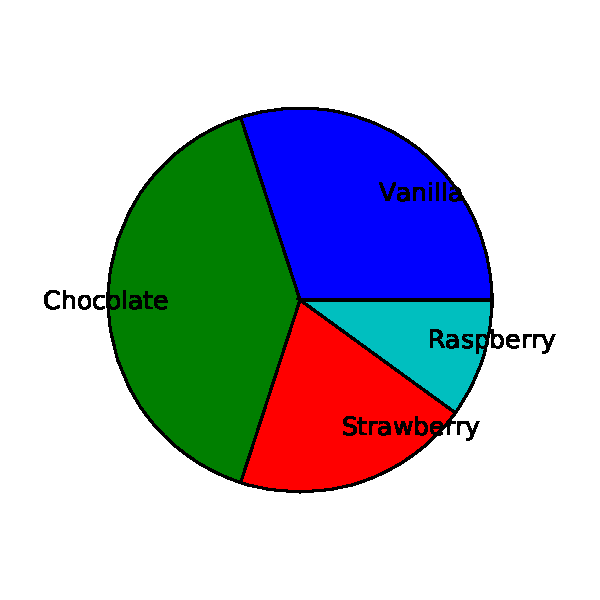
\includegraphics[width=0.6\textwidth]{Chapter-2/figs/pie}
\caption{Here is a sample figure}
\label{fig:hist1}
\end{figure}
%
\begin{figure}[hbtp]
\centering
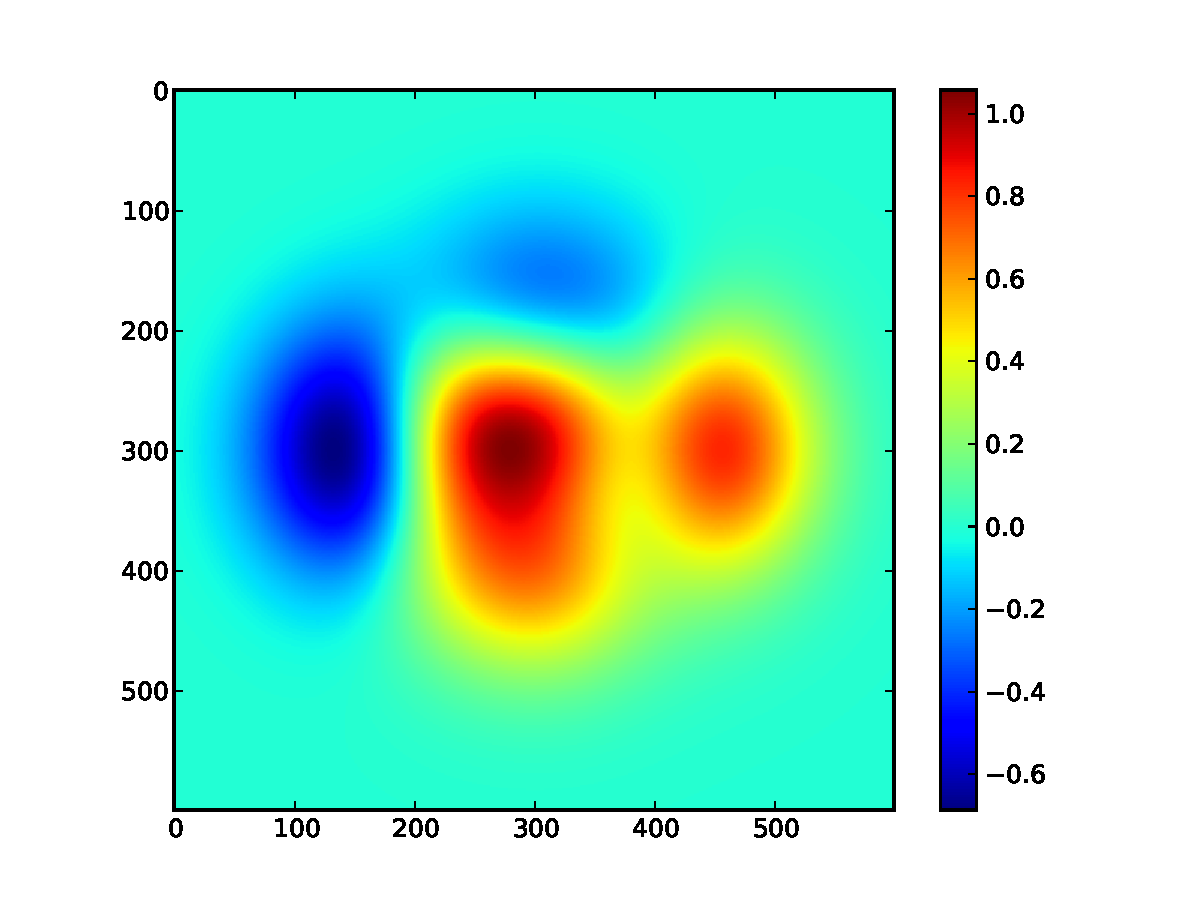
\includegraphics[width=0.6\textwidth]{Chapter-2/figs/color}
\caption{Here is a sample figure}
\label{fig:hist2}
\end{figure}

\paragraph{Filler Text} \lipsum[12-15]

\begin{lscape}
\begin{figure}
\centering
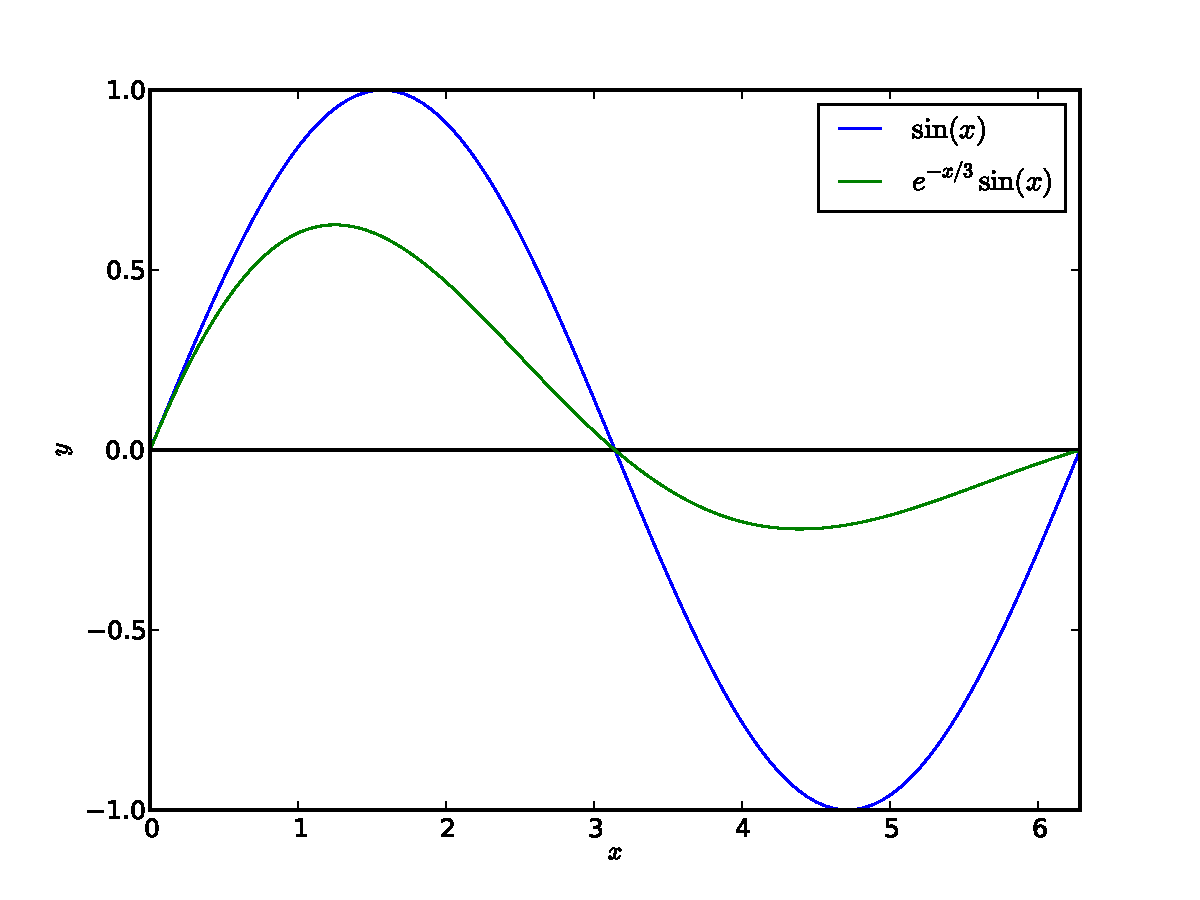
\includegraphics[width=\textwidth]{Chapter-2/figs/sine}
%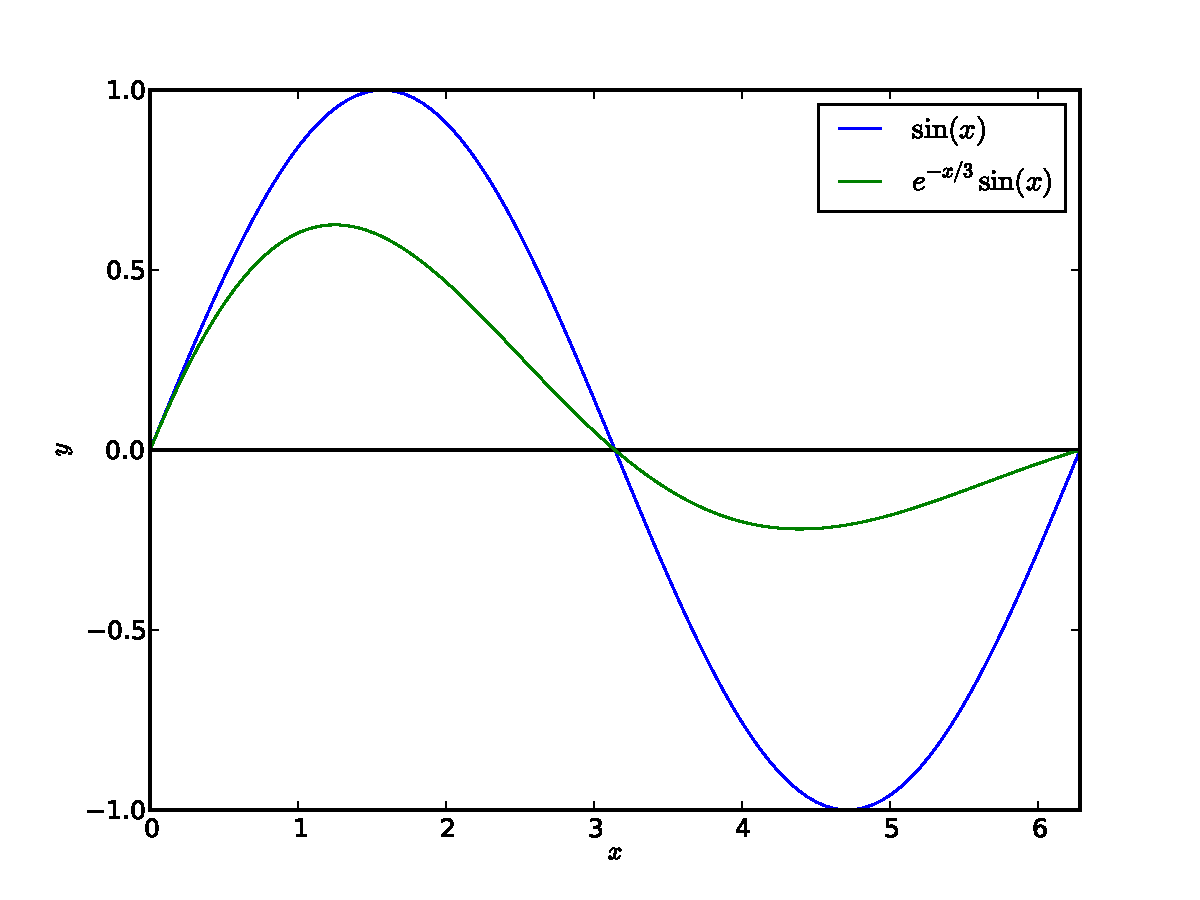
\includegraphics[height=\textwidth]{Chapter-2/figs/sine}
\caption{This figure has been turned sideways.  With large figures, 
         the author must ensure that there are at least two double spaces
         between the caption and the page number.}
\label{fig:hist}
\end{figure}
\end{lscape}

\section{Matrices}
Let's look at a simple example of a matrix:
\[ \left( \begin{array}{ccc}
a & b & c \\
d & e & f \\
g & h & i \end{array} \right)\] 
%
You may prefer to write it this way:
\[ \left[\begin{array} {cccccc}
1 & 0 & 0 & 0 & 0 & 0 \\
0 & 1 & 0 & 0 & 0 & 0 \\
0 & 0 & 1 & 0 & 0 & 0 \\
0 & 0 & 0 & 1 & 0 & 0 \\
0 & 0 & 0 & 0 & 1 & 0 \\
0 & 0 & 0 & 0 & 0 & 1 \\
\end{array} \right] \]

\chapter{Lorem Ipsum}

\section*{A First Section}

\paragraph{Filler Text} \lipsum[1-6]
%
\begin{figure}[t]
  \centering
  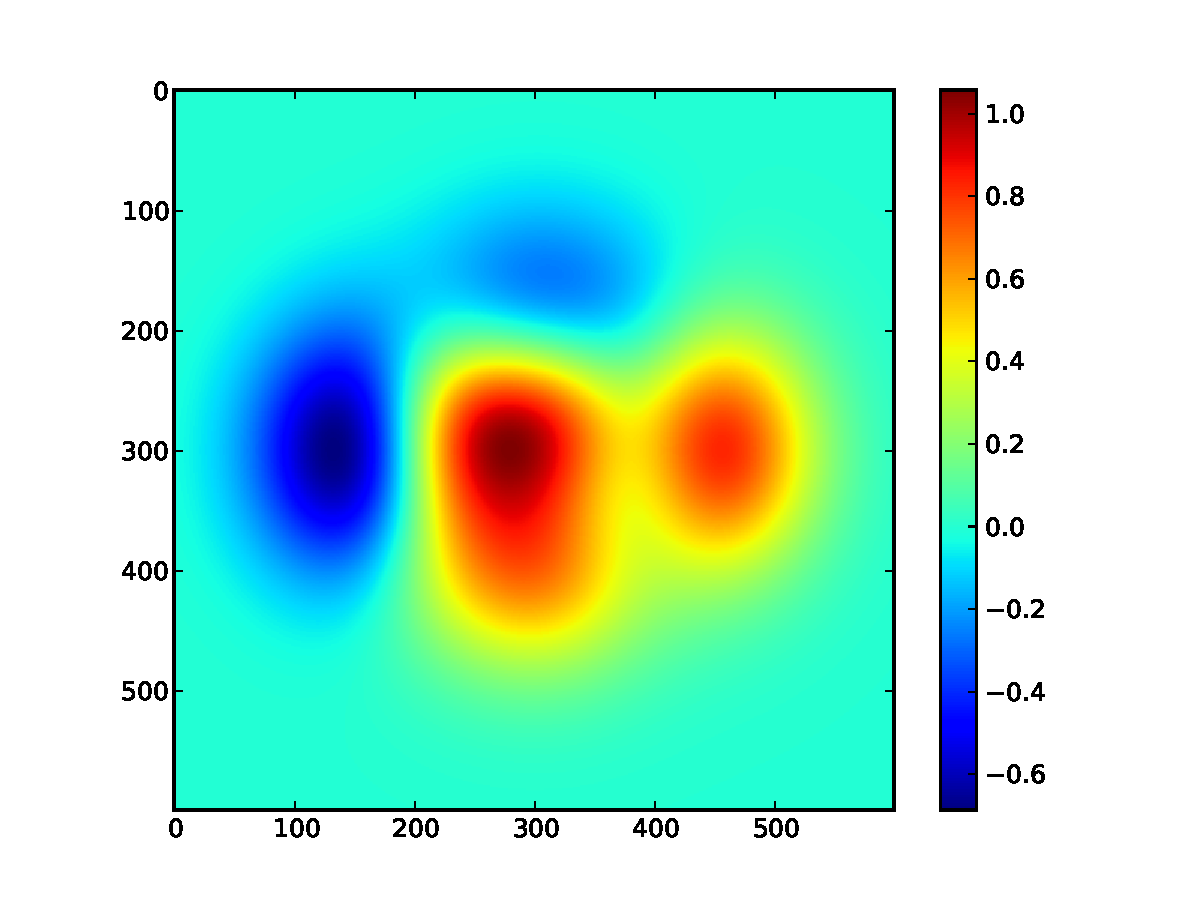
\includegraphics[width=0.6\textwidth]{Chapter-2/figs/color}
  \caption{A figure at the top of the page.}
  \label{fig:ch3.1}
\end{figure}
%
\lipsum[7-13]
%
\begin{figure}[!h]
  \centering
  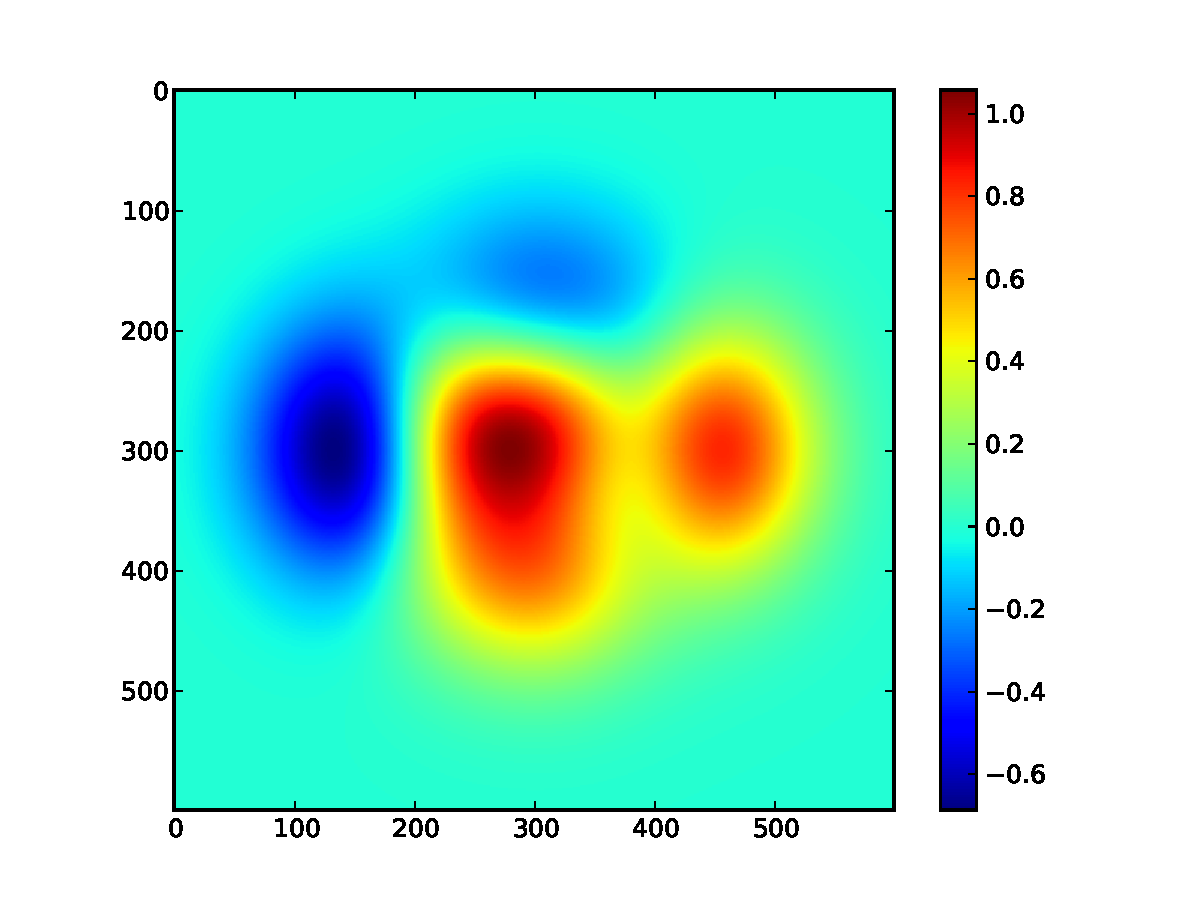
\includegraphics[width=0.6\textwidth]{Chapter-2/figs/color}
  \caption{A figure in the middle of text.}
  \label{fig:ch3.2}
\end{figure}
%
\begin{figure}[!b]
  \centering
  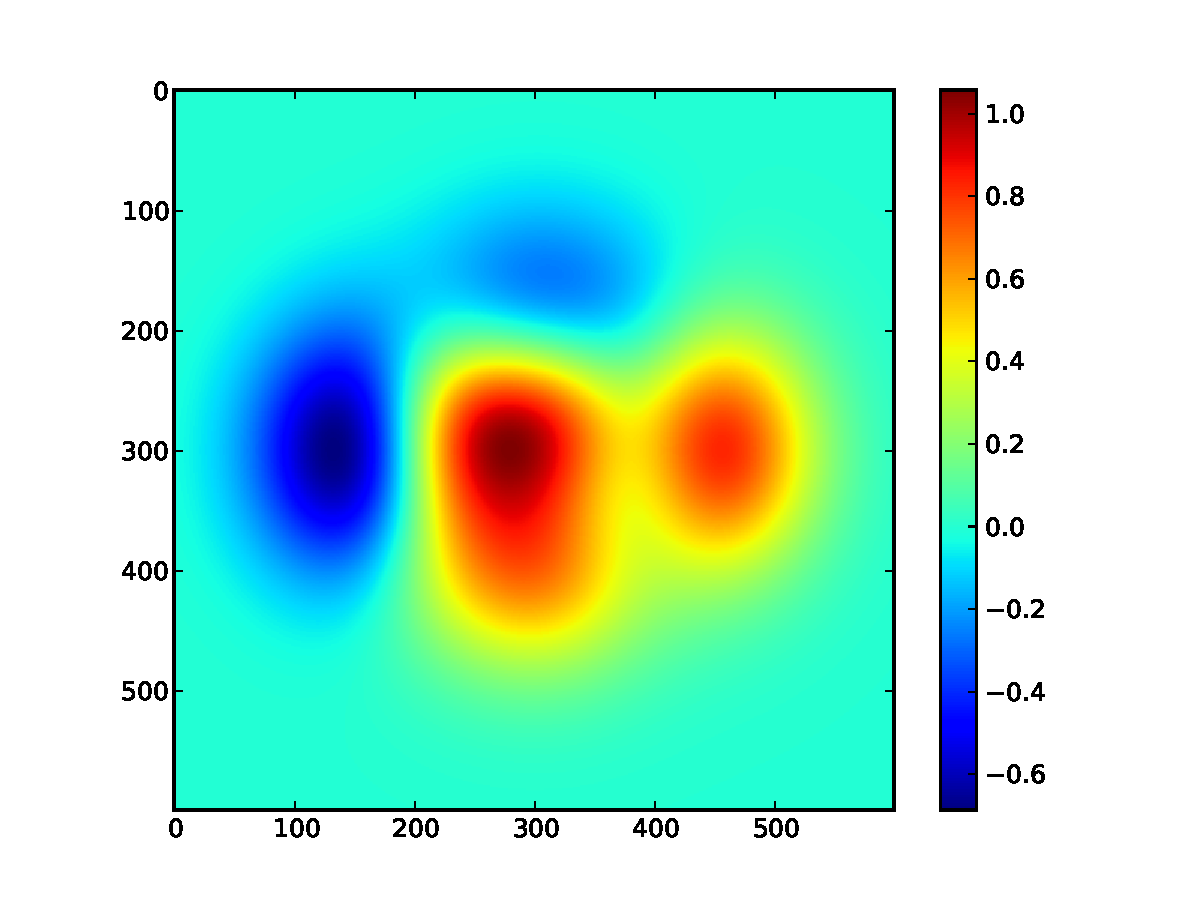
\includegraphics[width=0.6\textwidth]{Chapter-2/figs/color}
  \caption{A figure at the bottom of the page.}
  \label{fig:ch3.3}
\end{figure}
%
\lipsum[14-20]




%%---------------------------------------------------------------------------%%
%%--------------------------------- Bibliography ----------------------------%%
%%---------------------------------------------------------------------------%%
%%  You can use the bibitem list.
%\bibliographystyle{unsrt}
%\begin{thebibliography}{99}
%\bibitem{cb02}
%Casella, G. and Berger, R.L. (2002)
%\newblock {\it Statistical Inference, Second Edition.}
%Duxbury Press, Belmont, CA.
%
%\bibitem{t06}
%Tsiatis, A.A. (2006)
%\newblock {\it Semiparametric Theory and Missing Data.}
%Springer, New York.
%
%\end{thebibliography}

%% or use BibTeX
\bibliography{YourName-thesis}{}
\bibliographystyle{plain}

% Appendices
\appendix

\Appendix{Lorem Ipsum}

\section{A First Section}

\paragraph{Filler Text} \lipsum[1-6]
%
\begin{figure}
  \centering
  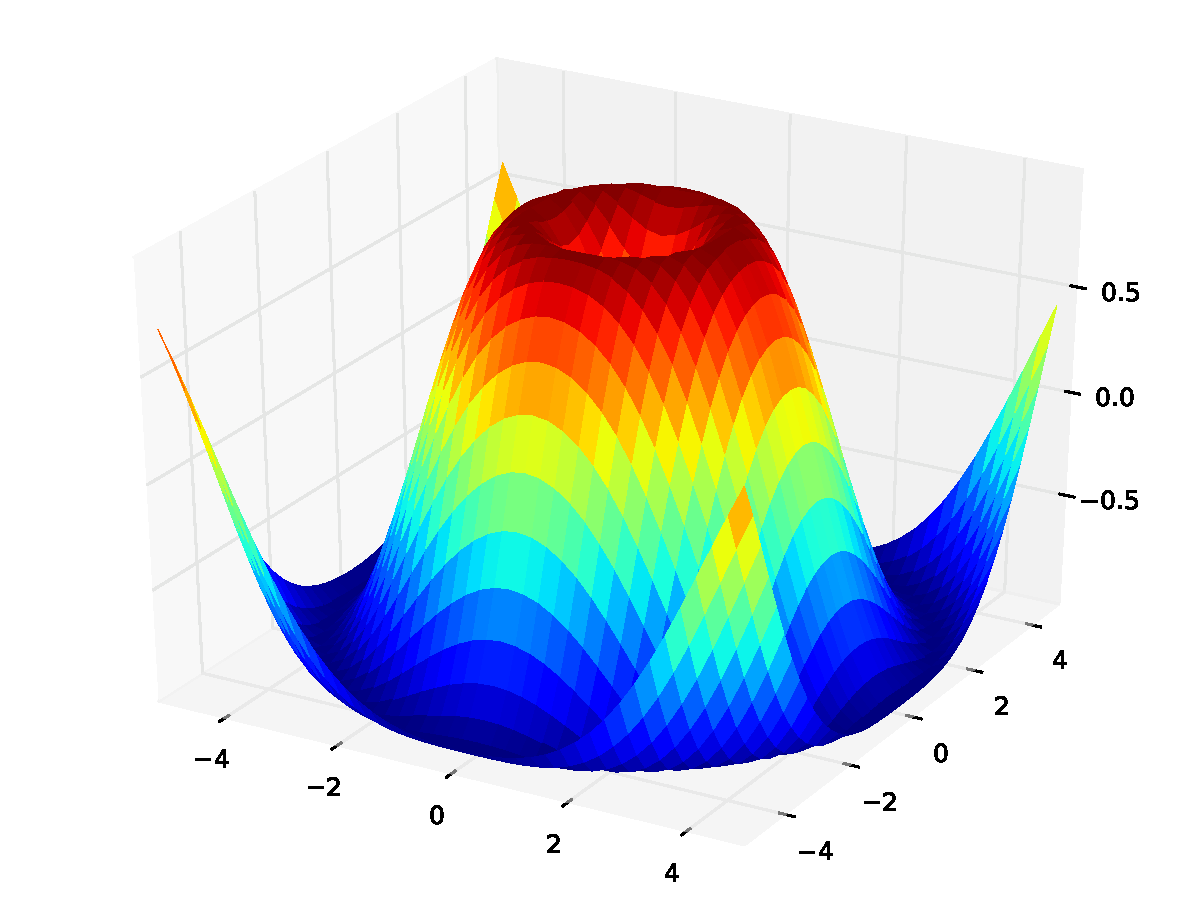
\includegraphics[width=0.6\textwidth]{Chapter-2/figs/threed}
  \caption{A figure in the appendix.}
  \label{fig:app}
\end{figure}
%
\lipsum[7-10]
\begin{table}
  \caption{A table in the appendix.}
  \label{tab:app}
  \begin{center}
    \begin{tabular}{lc}
      \toprule
      System & Author \\
      \midrule
      \TeX   & Donald Knuth   \\
      \LaTeX & Leslie Lamport \\
      \bottomrule
    \end{tabular}
  \end{center}
\end{table}
%

\section{A Second Section}

\lipsum[14-15]



%%---------------------------------------------------------------------------%%
\backmatter


\end{document}
